\documentclass[10pt,twocolumn]{article}
\usepackage[a4paper,margin=0.85in]{geometry}
\setlength{\columnsep}{0.28in}

\usepackage[T1]{fontenc}
\usepackage[utf8]{inputenc}
\usepackage{lmodern}
\usepackage{amsmath,amssymb}
\usepackage{booktabs}
\usepackage{array}
\usepackage{longtable}
\usepackage{graphicx}
\usepackage{tikz}
\usetikzlibrary{arrows.meta,positioning,fit,backgrounds,calc}
\usepackage{hyperref}
\hypersetup{
  colorlinks=true,
  linkcolor=black,
  citecolor=black,
  urlcolor=blue,
  pdftitle={ReproBot -- Second Progress Report},
  pdfauthor={Aleyna Kutuk, Engincan Varan, Gul Korkut, Goktug Mert Ozdogan}
}
\usepackage{xcolor}
\usepackage{caption}
\usepackage{pifont}

\definecolor{builtc}{HTML}{1B6F50}
\definecolor{missingc}{HTML}{97303F}
\definecolor{loopc}{HTML}{0E6E78}
\definecolor{warnc}{HTML}{97590C}

\newcommand{\built}{\textcolor{builtc}{\ding{51}}}
\newcommand{\absent}{\textcolor{missingc}{\ding{55}}}

\title{\textbf{ReproBot: A Multi-Agent System for Automated Scientific Paper Replication}\\[0.4em]
\large Second Progress Report}
\author{
  Aleyna Kütük \\ \small\texttt{aleynakutuk10@gmail.com}
  \and
  Engincan Varan \\ \small\texttt{engincanvaran@gmail.com}
  \and
  Gül Korkut \\ \small\texttt{serifegulkorkut@gmail.com}
  \and
  Göktuğ Mert Özdoğan \\ \small\texttt{goekmeroz@gmail.com}
}
\date{inzva AI Projects \#10 \\ 22.08.2026}


\begin{document}

\maketitle

\begin{abstract}
The first progress report described ReproBot as a proposed four-agent pipeline for
automated machine learning paper replication, supported by a literature review, an
implementation-ready project plan, and an early Reader prototype. This report covers the
implementation phase. Five of the seven planned components are now built and verified by
execution: PDF extraction, a five-field structured Reader, a Coder that emits a
self-contained training script, a Docker-sandboxed Runner, and an Orchestrator owning the
shared-memory state and the Coder\,$\leftrightarrow$\,Runner retry loop. Two papers --
\emph{Network In Network} and \emph{Wide Residual Networks} -- have been carried end to
end, from PDF through to a training script executing inside a container and reporting
metrics back. We report three substantive findings. First, the retry loop repairs real
defects: a deliberately reintroduced runtime fault was triaged, fed back to the Coder as
targeted feedback, and repaired on the first retry. Second, structured architecture
extraction measurably outranks the language model's pretrained priors -- given
\emph{Network In Network}, whose contribution is a custom \texttt{mlpconv} layer with no
memorized reference implementation, the Coder produced the correct layer cascade and
global-average-pooling head rather than the generic convolutional stack its priors would
favour. Third, several failure modes in LLM tool use are silent by construction and
require deterministic guards rather than prompt engineering. We are explicit about what
remains: the Critic does not exist, so no reproduced number has yet been compared against
any paper's claim, and the measured CPU throughput places a full-fidelity training run at
roughly 22 days per paper, making GPU access a precondition for any fidelity result.
\end{abstract}

\section{Introduction}
\label{sec:intro}

The first progress report \cite{reprobot2026first} established ReproBot's motivation and
design. The problem it addresses is unchanged: reproducing a machine learning paper's
empirical results is a mechanical task in principle and a labor-intensive one in
practice, and the large majority of published work ships no usable implementation --
across ICLR, ICML and NeurIPS 2024, only 16.7--21.2\% of accepted papers included a
working one \cite{seo2025papercoder}. The gap ReproBot targets is equally unchanged: no
surveyed system combines parsing a paper's claims, executing a faithful implementation,
and explicitly verifying the reproduced numbers against the published ones with a repair
loop driven by that comparison.

What has changed is that the system now exists in code. This report is therefore
structured around evidence rather than intent. Section~\ref{sec:architecture} describes
the architecture as implemented, and where it departs from the plan.
Section~\ref{sec:stages} documents each stage. Section~\ref{sec:results} reports the
measured results of running two papers through the full pipeline.
Section~\ref{sec:findings} collects engineering findings that we believe generalize
beyond this project. Section~\ref{sec:limitations} states the limitations plainly,
including the ones that prevent us from making any replication-fidelity claim at all.
Sections~\ref{sec:next} and \ref{sec:conclusion} cover next steps and conclusions.

Since the first report, the project has produced 30 commits across five newly implemented
pipeline stages totalling approximately 6{,}700 lines of Python, together with 21 logged
delegations to specialized coding, research, review and validation subagents.

\section{Implemented Architecture}
\label{sec:architecture}


\begin{figure*}[tbp]
\centering
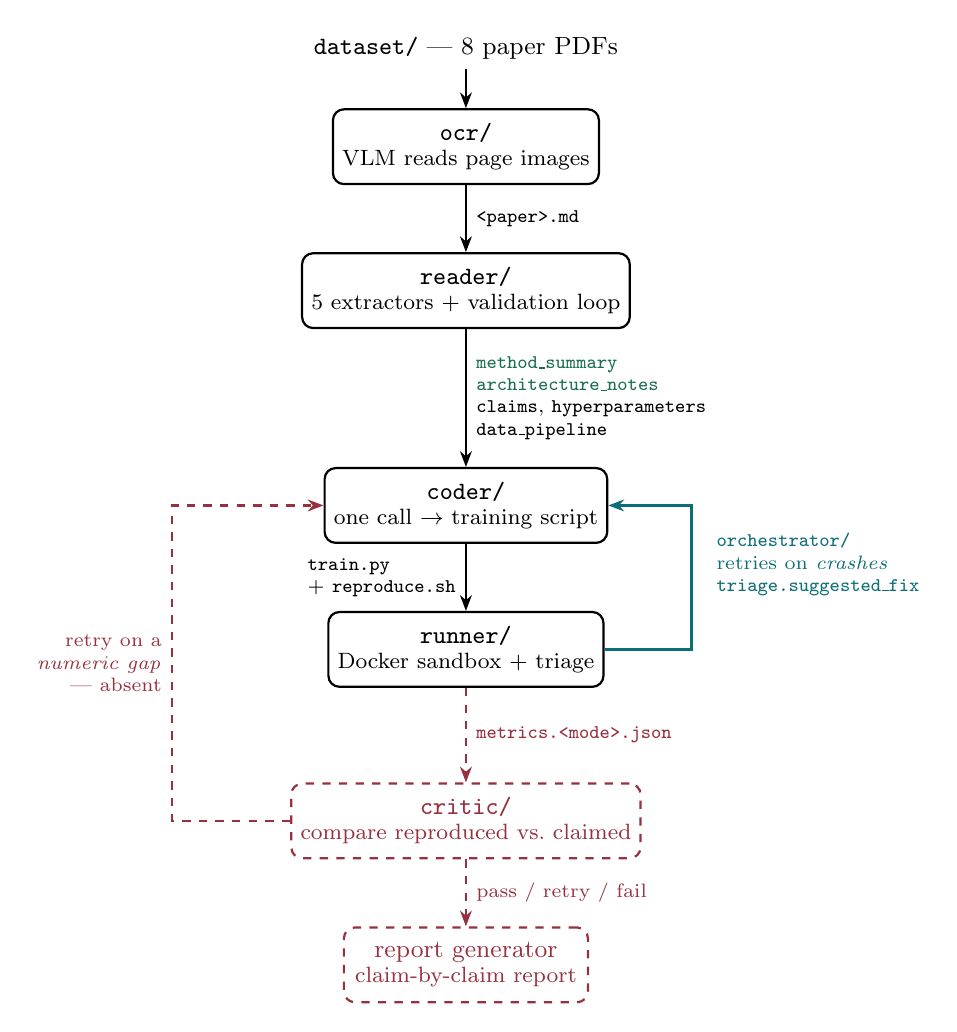
\begin{tikzpicture}[
  node distance=0.85cm and 1.5cm,
  stage/.style={draw, rounded corners, minimum width=3.1cm, minimum height=0.95cm,
    align=center, font=\small, thick},
  gone/.style={draw, rounded corners, minimum width=3.1cm, minimum height=0.95cm,
    align=center, font=\small, dashed, thick, draw=missingc, text=missingc},
  arr/.style={-{Stealth[length=2mm]}, thick},
  gonearr/.style={-{Stealth[length=2mm]}, thick, dashed, draw=missingc},
  looparr/.style={-{Stealth[length=2mm]}, very thick, draw=loopc},
  lbl/.style={font=\scriptsize, align=left},
  gonelbl/.style={font=\scriptsize, align=left, text=missingc}
]
  \node[stage] (ocr)    {\texttt{ocr/}\\[-2pt]\footnotesize VLM reads page images};
  \node[stage, below=of ocr] (reader) {\texttt{reader/}\\[-2pt]\footnotesize 5 extractors + validation loop};
  \node[stage, below=1.75cm of reader] (coder) {\texttt{coder/}\\[-2pt]\footnotesize one call $\to$ training script};
  \node[stage, below=of coder] (runner) {\texttt{runner/}\\[-2pt]\footnotesize Docker sandbox + triage};
  \node[gone,  below=1.2cm of runner] (critic) {\texttt{critic/}\\[-2pt]\footnotesize compare reproduced vs.\ claimed};
  \node[gone,  below=of critic] (report) {report generator\\[-2pt]\footnotesize claim-by-claim report};

  \node[above=0.5cm of ocr, font=\small] (pdf) {\texttt{dataset/} --- 8 paper PDFs};

  \draw[arr] (pdf) -- (ocr);
  \draw[arr] (ocr) -- node[right, lbl] {\texttt{<paper>.md}} (reader);
  \draw[arr] (reader) -- node[right, lbl]
    {\textcolor{builtc}{\texttt{method\_summary}}\\
     \textcolor{builtc}{\texttt{architecture\_notes}}\\
     \texttt{claims}, \texttt{hyperparameters}\\ \texttt{data\_pipeline}} (coder);
  \draw[arr] (coder) -- node[left, lbl] {\texttt{train.py}\\ + \texttt{reproduce.sh}} (runner);
  \draw[gonearr] (runner) -- node[right, gonelbl] {\texttt{metrics.<mode>.json}} (critic);
  \draw[gonearr] (critic) -- node[right, gonelbl] {pass / retry / fail} (report);

  % the real loop
  \draw[looparr] (runner.east) -- ++(1.1,0) |- (coder.east);
  \node[lbl, text=loopc, right=1.25cm of coder.east, anchor=west, yshift=-0.75cm]
    {\textbf{\texttt{orchestrator/}}\\ retries on \emph{crashes}\\ \texttt{triage.suggested\_fix}};

  % the absent loop
  \draw[gonearr] (critic.west) -- ++(-1.5,0) |- node[pos=0.25, left, gonelbl, align=right]
    {retry on a\\ \emph{numeric gap}\\ --- absent} (coder.west);
\end{tikzpicture}
\caption{ReproBot as implemented. Solid components are built and verified by execution;
dashed components in red do not exist. Two loops are shown and only one is real: the
Orchestrator retries on execution failures, routing the Runner's triage back to the Coder
as feedback. The absent loop --- retrying on a numeric gap between the reproduced value
and the paper's claim --- is the one the literature review identifies as missing from
every surveyed system, and it is missing here too.}
\label{fig:pipeline}
\end{figure*}


The pipeline follows the planned Reader\,$\to$\,Coder\,$\to$\,Runner shape, with two
departures worth stating.

\textbf{The Reader emits five fields, not four.} The project plan specified
\texttt{method\_summary}, \texttt{claims}, \texttt{hyperparameters} and
\texttt{architecture\_notes}. All four are implemented. A fifth,
\texttt{data\_pipeline}, was added on the plan's own recommendation: data-processing
detail is the single weakest-covered aspect of paper-to-code extraction across every
surveyed system (56\% coverage in PaperCoder against 79--92\% elsewhere
\cite{seo2025papercoder}), and is therefore treated as a first-class output field rather
than folded into the method summary.

\textbf{The Runner's interface is a generated shell script, not a command line.} The
Coder emits a \texttt{reproduce.sh} alongside every training script, exposing four modes
--- \texttt{probe}, \texttt{smoke}, \texttt{capped} and \texttt{full} --- and the Runner
invokes nothing else. It never constructs a Python command and never passes a flag. This
keeps the Runner paper-agnostic: a future paper whose script requires entirely different
arguments changes only its own \texttt{reproduce.sh}. The contract narrows from eight
exactly-spelled command-line flags to four mode names.

The Orchestrator is implemented as a bounded, deterministic Python loop rather than the
LangGraph state machine the plan proposed. At the present scope the graph would comprise
three nodes and one conditional edge, which does not justify the dependency. The
shared-memory object follows the plan's schema exactly and the transition logic is
isolated in pure functions, so migration remains mechanical once the Critic introduces
genuine branching.

\section{Stage Implementations}
\label{sec:stages}

\subsection{Extraction: \texttt{ocr/}}

Four independent PDF-to-Markdown backends share one command-line shape. The
vision-language backend renders each page to an image and sends it to Claude, so figures
are genuinely read rather than inferred from surrounding text --- a property the Reader's
architecture extraction depends on directly (Section~\ref{sec:reader}). Six of the eight
target papers are extracted. Two fail on a deterministic content-filter false positive,
diagnosed as originating in the vision classifier rather than in our prompt: the same
page fails identically at different render scales and under a minimal one-line prompt.

\subsection{Structured extraction: \texttt{reader/}}
\label{sec:reader}

Five extractors implement a shared abstract base class, so the pipeline treats every
stage uniformly and a new extraction type requires one new class and one line in the
stage list. A validator makes one further model call over the combined output and the
paper text, flagging inconsistencies without fixing them; the pipeline routes each flag
back to the single stage its \texttt{relates\_to} prefix names, re-runs that stage with
the flag folded into its prompt as feedback, and re-validates, capped at three passes.

Two properties of \texttt{architecture\_notes} proved load-bearing.

\textbf{Recording what the paper does not say.} The field \texttt{unstated\_details} is
required, not optional. \emph{Network In Network} describes three \texttt{mlpconv} layers
and a global average pooling layer in prose and in its Figure~2, but never states filter
counts, kernel sizes or strides in the main text, deferring them to supplementary
material. The extractor records twelve such gaps, quoting the paper's own deferral, and
invents no values. This matters more here than elsewhere in the pipeline: code has to
run, so a confidently invented channel count does not fail loudly --- it trains the wrong
network and reports a number for it.

\textbf{Distinguishing the paper's own equations from its contrasts.} A paper introducing
a new layer typically prints the conventional formulation, and often a rival's, beside its
own. \emph{Network In Network} prints all three within two pages. Returned as an
undifferentiated list, these are three plausible specifications and a code generator will
implement one of them. Instructing the model to omit baseline equations did not work; it
continued to return them. Requiring the \emph{schema} to carry an
\texttt{is\_own\_method} flag on every entry did work, and the distinction survives into
the generated code.

\subsection{Code generation: \texttt{coder/}}

One model call converts a paper's Reader output plus its Markdown into a self-contained
HuggingFace \texttt{Trainer} script. Input precedence is explicit and ordered:
\texttt{architecture\_notes} first, the paper text as corroboration, and the model's own
recollection last and only when disclosed in the output's \texttt{assumptions} field.

Two deterministic gates run before a script is accepted, both free of model calls.
The script must parse as valid Python, and every flag the Runner depends on must
literally appear in its text. Neither gate can establish that the script \emph{runs} ---
a limitation that recurs in Section~\ref{sec:findings}.

\subsection{Sandboxed execution: \texttt{runner/}}

The generated script executes inside a Docker container built from a pinned CPU-only
image. Stages escalate and stop at the first failure. Timeout enforcement required care:
terminating the client process leaves the container running under the daemon, so every
run is launched with an explicit name and killed by that name on expiry.

A single cheap model call triages a genuine failure into \emph{recoverable} --- a defect
in the generated script --- or \emph{environmental}. Success and timeout are classified
mechanically with no model call at all, which both saves cost on the common path and
avoids inviting a judgment where the exit status already answers the question.

\subsection{The retry loop: \texttt{orchestrator/}}

The Orchestrator owns the shared-memory object and the loop. Its routing order is
deliberate: an environmental error stops immediately rather than consuming retries,
because regenerating a script cannot repair a broken container. A timeout likewise stops,
since no triage is produced for timeouts by design and a slow but correct script must not
be ``repaired'' into a different one. Only a recoverable error regenerates.

A plateau guard compares each regenerated script against its predecessor and stops early
when they are near-identical, rather than exhausting the budget on a fix that is not
changing anything --- following PaperBench's observation that agents plateau rather than
making steady long-horizon progress \cite{starace2025paperbench}.


\begin{figure*}[tbp]
\centering
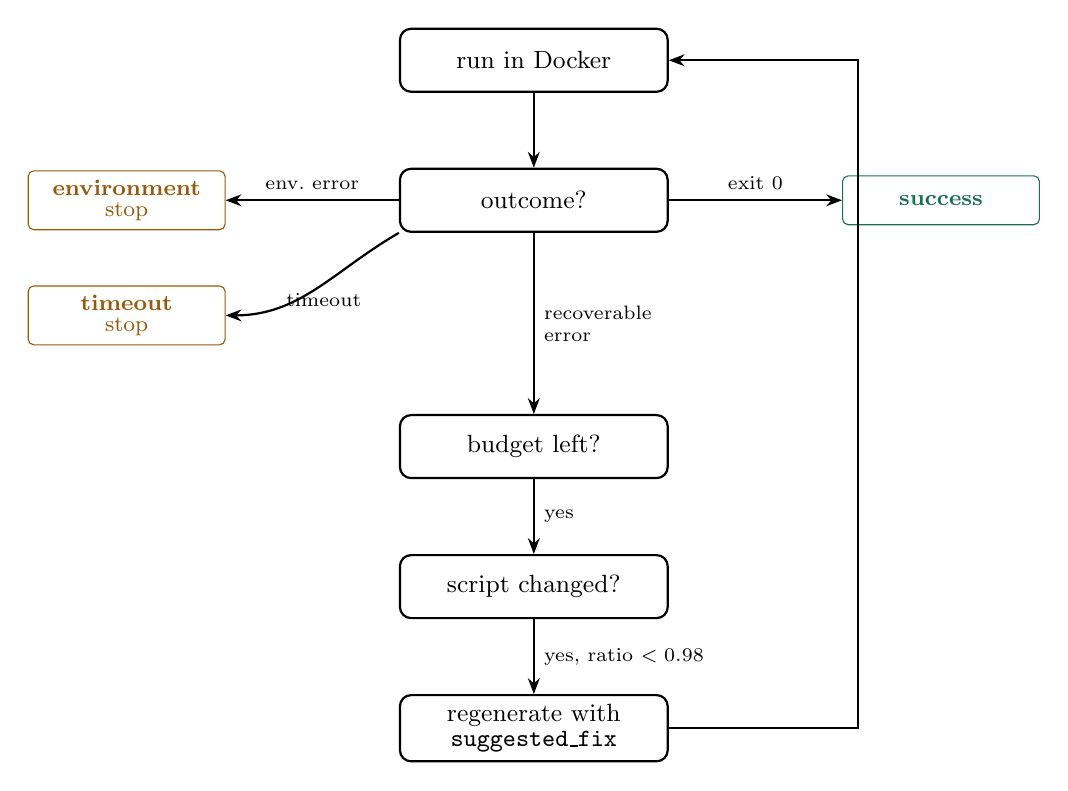
\begin{tikzpicture}[
  dec/.style={draw, rounded corners, minimum width=3.4cm, minimum height=0.8cm,
    align=center, font=\small, thick},
  term/.style={draw, rounded corners=2pt, minimum width=2.5cm, minimum height=0.62cm,
    align=center, font=\footnotesize},
  arr/.style={-{Stealth[length=2mm]}, thick},
  lbl/.style={font=\scriptsize}
]
  \node[dec] (run) {run in Docker};
  \node[dec, below=0.95cm of run] (status) {outcome?};
  \node[dec, below=2.3cm of status] (budget) {budget left?};
  \node[dec, below=0.95cm of budget] (plateau) {script changed?};
  \node[dec, below=0.95cm of plateau] (regen) {regenerate with\\[-2pt]\texttt{suggested\_fix}};

  \node[term, right=2.2cm of status, draw=builtc, text=builtc] (ok) {\textbf{success}};
  \node[term, left=2.2cm of status, draw=warnc, text=warnc] (env) {\textbf{environment}\\[-2pt]stop};
  \node[term, below=0.7cm of env, draw=warnc, text=warnc] (to) {\textbf{timeout}\\[-2pt]stop};

  \draw[arr] (run) -- (status);
  \draw[arr] (status) -- node[above, lbl] {exit 0} (ok);
  \draw[arr] (status) -- node[above, lbl] {env.\ error} (env);
  \draw[arr] (status.south west) to[out=210, in=0] node[below, lbl, pos=0.45] {timeout} (to.east);
  \draw[arr] (status) -- node[right, lbl, align=left] {recoverable\\ error} (budget);
  \draw[arr] (budget) -- node[right, lbl] {yes} (plateau);
  \draw[arr] (plateau) -- node[right, lbl] {yes, ratio $<0.98$} (regen);
  \draw[arr] (regen.east) -- ++(2.4,0) |- (run.east);
\end{tikzpicture}
\caption{The Orchestrator's routing. The order is deliberate: an environmental error stops
\emph{before} the retry budget is consulted, because regenerating a script cannot repair a
broken container. A timeout also stops rather than retrying --- no triage is produced for
timeouts by design, and a slow but correct script must not be ``repaired'' into a
different one. Only a recoverable error, within budget, whose regenerated script actually
differs from its predecessor, results in another execution.}
\label{fig:loop}
\end{figure*}


\section{Results}
\label{sec:results}

\subsection{Extraction coverage}

Table~\ref{tab:reader} reports the Reader's output across the four papers processed. The
\emph{own/eq} column is the most informative: it counts equations marked as the paper's
own against the total captured. \emph{All Convolutional Net} prints six equations of
which two are its own; \emph{Wide Residual Networks} prints one and it is its own. A
field that always returned every equation would be useless to a code generator.

\begin{table}[htbp]
\centering
\small
\caption{Reader output across four papers. \emph{Comp.} is architecture components;
\emph{own/eq} is own-method equations over equations captured; \emph{Gaps} is
\texttt{unstated\_details} entries; \emph{Flags} is unresolved validation flags after the
three-pass cap.}
\label{tab:reader}
\begin{tabular}{lrrrrcrr}
\toprule
Paper & Claims & Hyp. & Data & Comp. & own/eq & Gaps & Flags \\
\midrule
Network In Network      & 12 & 17 & 4 &  7 & 1/3 & 12 & 4 \\
All Convolutional Net   & 17 & 13 & 4 & 10 & 2/6 & 11 & 5 \\
Deep Residual Learning  & 66 & 28 & 6 & 10 & 2/3 &  7 & 8 \\
Wide Residual Networks  & 61 & 20 & 4 & 11 & 1/1 & 11 & 6 \\
\bottomrule
\end{tabular}
\end{table}

Validation does not converge. Every paper finishes with flags remaining after the cap,
and the count is worst on the paper with the most claims. Inspection shows a substantial
proportion are the validator raising a concern and dismissing it within its own
description rather than identifying a real defect. We regard this as a genuine limitation
of the current design rather than a tuning problem, and record it as such.

\subsection{End-to-end execution}

Both papers with generated scripts were carried through the Orchestrator. Both succeeded
on the first attempt with no retries required (Table~\ref{tab:runs}).

\begin{table}[htbp]
\centering
\small
\caption{End-to-end runs. Both papers reached \texttt{smoke} and returned
\texttt{success} with zero retries consumed. Reproduced values are reported to
demonstrate that the measurement path works end to end; they are \emph{not}
replication results (Section~\ref{sec:limitations}).}
\label{tab:runs}
\begin{tabular}{lrrrr}
\toprule
Paper & probe & smoke & Reproduced & Claimed \\
\midrule
Network In Network     &  32.2\,s &  62.1\,s & 86.72\% & 10.41\% \\
Wide Residual Networks & 241.4\,s & 367.2\,s & 89.45\% &  4.00\% \\
\bottomrule
\end{tabular}
\end{table}

The roughly sixfold difference in wall clock reflects model size: WRN-28-10 carries
approximately 36.5M parameters against \emph{Network In Network}'s order of 1M. The
reproduced error rates are far from the claimed values, and this is the expected and
correct behaviour of the stages that produced them --- \texttt{probe} and \texttt{smoke}
train for one epoch over a few hundred images and exist to answer whether the script
runs, never whether the number is right.

\subsection{The retry loop repairs real defects}

The loop was validated against a deliberately reintroduced fault: a learning-rate
scheduler whose method reads an attribute its constructor never assigns. The fault is
valid Python, so the syntax gate admits it, and it raises only when the training loop
first logs the learning rate. This is precisely the class of defect the loop exists for.

The container run failed with an \texttt{AttributeError}; triage classified it as
recoverable and produced a targeted fix naming the class and the missing assignment; the
Coder regenerated with that text folded into its prompt; the plateau guard measured a
similarity of 0.41 against the previous attempt, well below the 0.98 stopping threshold;
and the second attempt passed. The repair was not incidental --- the regenerated script
retained the class the triage named and added exactly the missing assignment.

This is the local counterpart of AutoReproduce's ablation, in which removing the
debug loop barely moved an LLM-judged alignment score while nearly tripling the
performance-gap metric \cite{zhao2025autoreproduce}: code can read as a faithful
implementation and still be wrong if it is never executed.

\subsection{Architecture extraction outranks pretrained priors}

The Coder was verified against \emph{Network In Network} rather than \emph{Wide Residual
Networks}, deliberately. A wide residual network is among the most thoroughly memorized
architectures in the literature and would be reproduced correctly from priors alone,
demonstrating nothing about the extraction. \emph{Network In Network} is the honest test:
its \texttt{mlpconv} layer is the paper's contribution, its dimensions appear nowhere in
the paper, and its equation list contains two decoys.

The generated script contains a genuine \texttt{mlpconv} cascade --- a $k\times k$
convolution followed by two $1\times1$ convolutions, with a docstring mapping each line
to the paper's Equation~2 --- and contains no fully-connected layer at all, retaining the
global-average-pooling classifier that is the paper's second contribution. Both decoy
equations are explicitly excluded and named as excluded.

The strongest evidence is negative. A priors-driven implementation of this paper is a
plain convolutional stack with a fully-connected head; both of those defaults were
avoided, and the generated script justifies the avoidance by citing components tagged
\texttt{[baseline, not own method]} --- a label from our extraction schema, not language
from the paper.

We qualify this in one respect. The channel widths in the generated model are the
canonical configuration, drawn from the model's own knowledge rather than from the paper,
which genuinely omits them. This is the designed outcome and it is disclosed in the
output. The change made those values \emph{visible} rather than \emph{correct}, and a
Critic will need to weight a disclosed prior below a paper-sourced value.

\section{Engineering Findings}
\label{sec:findings}

\subsection{Silent failure modes in structured tool use}

Three distinct failure modes were observed in which a model call returns a structurally
valid response that is nonetheless empty or wrong, in a way indistinguishable from a
correct extraction over a paper that had nothing to report.

The first is output truncation at the token limit, which yields a partial payload.
The second is an intermittent well-formed response with every required field absent.
The third is the most instructive: a \emph{double-encoded} payload, in which the model
returns a clean tool-use response whose single key holds the entire result re-encoded as
a JSON string. Field lookups then all miss and the extraction is discarded. It reproduced
three times out of three on one paper, and fired again during later verification, where
without the guard it would have reported zero datasets on an apparently clean run.

All three are now handled in one shared module rather than at six call sites. The general
lesson is that structured-output failures do not necessarily announce themselves as
errors, and a pipeline that treats a well-formed empty response as a legitimate negative
result will silently accumulate them.

\subsection{Schemas constrain models more reliably than instructions}

Two independent cases: instructing the model to omit baseline equations did not stop it
returning them, whereas requiring a per-entry \texttt{is\_own\_method} flag produced
correct classification immediately; and a bookkeeping field the model never populated,
despite being schema-required on every run, was eliminated by deriving it from data
already present rather than by asking more insistently. Where a value is computable from
what has already been extracted, computing it is more reliable than requesting it.

\subsection{Static gates cannot establish that generated code runs}

Two defects reached generated scripts that passed every deterministic gate. The first is
the scheduler fault described above. The second, found by inspection, is a divergence
between a script's own bookkeeping --- which describes one stage as $192\to192\to10$ ---
and the code it emitted, which builds $192\to10\to10$. The script runs, and the choice is
a defensible reading of a dimension the paper never states; what is wrong is that the
record describes a different network from the code.

Neither is reachable by parsing. Both argue for the execution-driven loop rather than for
additional static analysis.

\subsection{Platform constraints shaped the architecture}

The development machine is an Intel Mac, and no PyTorch release supports both Python 3.13
and Intel macOS: 3.13 support arrived in the same release range that dropped Intel-macOS
wheels. Reducing to Python 3.11 installs PyTorch 2.2.2, but current \texttt{transformers}
requires 2.5 or newer and, on finding an older version, silently disables its PyTorch
backend rather than raising.

This is why the Runner executes inside a container rather than on the host. The container
runs its own Linux Python, so the constraint does not apply within it, and the project's
dependency lock stays free of PyTorch entirely.

\section{Limitations}
\label{sec:limitations}

We state these directly, because several bear on how the results above should be read.

\textbf{No fidelity claim is possible yet.} The Critic does not exist. Nothing in the
system compares a reproduced number against a paper's claim, and the field reserved for
that verdict is permanently null. The reproduced error rates in Table~\ref{tab:runs}
demonstrate that the measurement path works; they are not replication results and should
not be read as any.

\textbf{Full-fidelity runs are not currently feasible.} Measured throughput is 5.256
training samples per second for WRN-28-10 on this CPU. The paper's setup is 50{,}000
samples over 200 epochs, placing one paper and one claim at approximately 22 days. Every
result reported here comes from stages that train for one epoch over a few hundred
images. GPU access is a precondition for any fidelity measurement, not an optimization.

\textbf{The evidence base is two papers.} Both succeeded on the first attempt, so the
retry loop's behaviour in production remains demonstrated only by the injected fault.
Four of the loop's seven terminal verdicts have been exercised only against test doubles.

\textbf{Retries regenerate rather than patch.} A repair rewrites the whole file, so a
successful fix can introduce a new defect elsewhere, and nothing compares the semantics of
successive attempts. AutoReproduce's line-range edit mechanism
\cite{zhao2025autoreproduce} is the natural remedy and is not yet implemented.

\textbf{Validation does not converge}, as reported in Section~\ref{sec:results}, and two
of the eight target papers cannot currently be extracted at all.

\section{Next Steps}
\label{sec:next}

\textbf{The Critic} is the highest-value remaining component and closes the loop the
project's thesis rests on. Its verdict logic should remain simple, auditable arithmetic
against an explicit numeric tolerance rather than a model judging numbers by eye ---
Agent Laboratory's automated reviewer overestimated quality by 2.3 points against human
judges \cite{schmidgall2025agentlab}, and an objective numeric check is precisely the
failure mode ReproBot exists to avoid. It can be built and tested against synthetic
metrics immediately; its verdicts become meaningful when compute allows a real run.

\textbf{GPU compute} should be secured in parallel rather than afterwards, since it gates
every fidelity result.

\textbf{Coverage} should be extended across the remaining papers, which requires no new
code and would convert single demonstrations into distributions.

\textbf{The Report Generator} is the promised deliverable and the cheapest remaining
component: the shared-memory object already carries everything it needs, including the
append-only history log.

\section{Conclusion}
\label{sec:conclusion}

ReproBot has moved from design to a working pipeline. Five of seven components are
implemented and verified by execution; two papers have been carried from PDF to a
training script running in a sandbox; the retry loop repairs real defects; and structured
architecture extraction demonstrably outranks the language model's priors on a paper
where those priors would otherwise dominate.

What has been demonstrated is that the machinery works end to end. What has not been
demonstrated --- and cannot be, until the Critic exists and compute allows a full training
run --- is replication fidelity, which is the project's actual claim. We regard stating
that distinction clearly as more useful than reporting an aggregate that would obscure it.

\bibliographystyle{plain}
\begin{thebibliography}{9}

\bibitem{reprobot2026first}
Kütük, A., Varan, E., Korkut, G., \& Özdoğan, G.~M. (2026).
ReproBot: A Multi-Agent System for Automated Scientific Paper Replication --- First
Progress Report. \textit{inzva AI Projects \#10}.

\bibitem{starace2025paperbench}
Starace, G., Jaffe, O., Sherburn, D., Aung, J., et al. (2025).
PaperBench: Evaluating AI's Ability to Replicate AI Research.
\textit{arXiv:2504.01848}.

\bibitem{seo2025papercoder}
Seo, M., Baek, J., Lee, S., \& Hwang, S.~J. (2025).
Paper2Code: Automating Code Generation from Scientific Papers in Machine Learning.
\textit{arXiv:2504.17192}.

\bibitem{zhao2025autoreproduce}
Zhao, X., Sun, M., Wang, W., et al. (2025).
AutoReproduce: Automatic AI Experiment Reproduction with Paper Lineage.
\textit{arXiv:2505.20662}.

\bibitem{lin2025autop2c}
Lin, Z., Li, M., Chen, S., et al. (2025).
AutoP2C: An LLM-Based Agent Framework for Code Repository Generation from Multimodal
Content in Academic Papers. \textit{arXiv:2504.20115}.

\bibitem{schmidgall2025agentlab}
Schmidgall, S., Su, Y., Wang, Z., et al. (2025).
Agent Laboratory: Using LLM Agents as Research Assistants.
\textit{arXiv:2501.04227}.

\bibitem{li2024mlrcopilot}
Li, R., Patel, T., Wang, Q., \& Du, X. (2024).
MLR-Copilot: Autonomous Machine Learning Research based on Large Language Models Agents.
\textit{arXiv:2408.14033}.

\end{thebibliography}

\end{document}
